\documentclass{beamer}
\usepackage[romanian]{babel}
\usepackage[utf8]{inputenc}
\usepackage{graphicx}
\graphicspath{ {./images/} }

\title{Metode de analiză a circuitelor}
\author{Dinu Mihai Dinel}
\date{}


\begin{document}
\begin{frame}
\maketitle
\end{frame}



\begin{frame}{Introducere}
\par Un circuit electric/electronic este un sistem compus din elemente electronice, cum ar fi rezistențe, tranzistoare, condensatoare, inductori, diode și multe altele, conectate prin fire prin care poate circula curentul electric.
\par Analiza de circuit este analiza matematică a unui circuit electric sau electronic. Este procesul de studiu și analiză a mărimilor electrice prin calcule. Prin această analiză, putem găsi elementele necunoscute ale unui circuit, cum ar fi tensiunea, intensitatea, rezistența, impedanța, puterea. Când facem analiza circuitelor, trebuie să înțelegem mărimile electrice, relațiile, teoremele și unele legi esențiale.
\end{frame}


\begin{frame}{Analiza Nodala}
    \par Analiza nodală oferă o procedură generală pentru analiza circuitelor folosind tensiunile din noduri ca variabile de circuit. Alegerea tensiunilor de pe noduri în detrimentul tensiunilor elementelor ca variabile de circuit este mai convenabilă și reduce numărul de ecuații care trebuie să fie rezolvate simultan.
    Pașii de determinare a tensiunilor de pe noduri:

    \begin{figure}[h]
    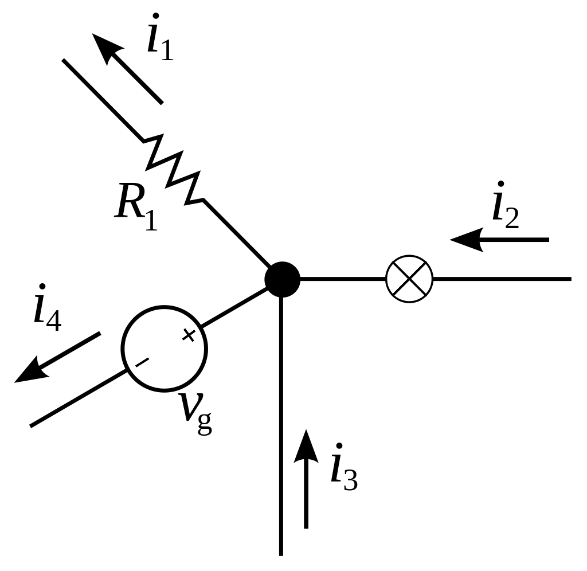
\includegraphics[width=3cm]{fig1.png}
    \centering
    \caption{Suma intensităților curenților care intră într-un nod de rețea este egală cu suma intensităților curenților care ies din același nod. \(i1 + i4 = i2 + i3\)}
    \end{figure}
\end{frame}

\begin{frame}{Analiza Ochiurilor}
\par Analiza ochiurilor oferă o altă procedură generală pentru analizarea circuitelor, utilizând curenții rețelei ca variabile ale circuitului. Utilizarea curenților din ochiuri în loc de curenții elementelor ca variabile de circuit este convenabilă și reduce numărul de ecuații care trebuie rezolvate simultan.

\begin{figure}[h]
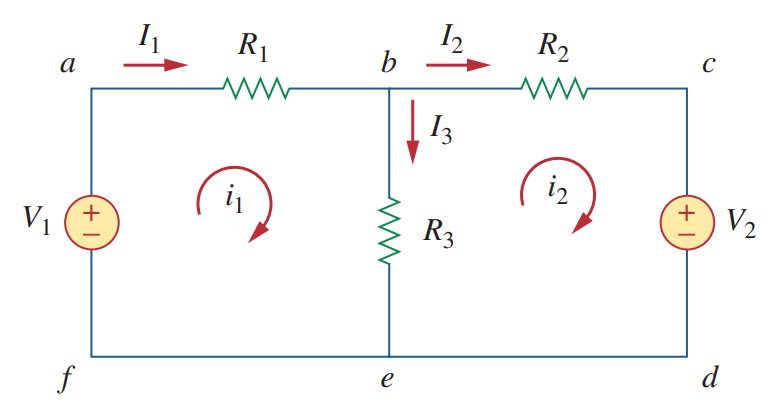
\includegraphics[width=3cm]{fig2.png}
\centering
\end{figure}

\par A doua lege a lui Kirchhoff:
\[\sum E_n=\sum{R_nI_n}\]
\[\sum V_n=0\]
\end{frame}


\begin{frame}{Concluzii}
Din cele prezentate anterior, observam ca metodele de analiza a ochiurilor sunt ușor de aplicat, iar asta reprezintă un avantaj important, ce poate însemna, printre altele, ca pot fi implementate ușor în programe de calculator care sa automatizeze acest proces.
\end{frame}


\begin{frame}{Bibliografie}
\begin{enumerate}
    \item Legile lui Kirchhoff – Wikipedia
    \item Fundamentals of Electric Circuits – Charles K. Alexander & Matthew
\end{enumerate}
\end{frame}

\end{document}

